
	\section{ACM/ICPC World Finals 2010}
		\subsection{ACM/ICPC World Finals 2010 B Barcodes}
			\subsubsection{题目大意}
				条形码能对 0 到 9,横杠 – 编码。如下表
				\begin{table}[!htb]
					\centering
					\begin{tabular}{ccccccccccc}
						\toprule
							符号 & 编码&&符号 & 编码 && 符号 & 编码&&符号 & 编码   \\
						\midrule
							0 & 00001 && 3 & 11000 && 6 & 01100 & & 9 & 10000 \\
							1 & 10001 && 4 & 00101 && 7 & 00011 && – & 00100 \\
							2 & 01001 && 5 & 10100 && 8 & 10010 && 起/止 & 00110 \\
						\bottomrule
					\end{tabular}
					\caption{编码}
				\end{table}
				
				其中 0 表示细线,1 表示粗线,是 0 粗细的\emph{两倍},颜色交替出现。最后还有两位校验码,计算方法在题面中已给出,并且首尾还需加上起止码。输入扫描器识别到的线的粗细,并容忍 $5 \%$ 的长度误差,请尝试识别信息,并返回返回正确的解码信息,或告知系统校验码错误,或根本无法识别。
				
				线段的条数 $N \le 150$。$1 \le $ 粗细 $ \le 200$。

			\subsubsection{算法讨论}
				如果已经识别出来孰粗孰细,那么接下来就确认方向。由于起止码不对称,故方向是很好确定的。随后按照编码解码,计算校验码,并返回结果即可。下述如何识别粗细。
				
				一个正确的条形码中粗的和细的条纹都出现过(至少起止码里就有)。那么最粗的长度 $Max$ 肯定是 1,最细的 $Min$ 肯定是 0。设 0 的参考粗细为 $a$,那么
				\begin{align}
					x \text{ 表示细条}, \quad \quad & \frac{19}{20} \, a \le x \le \frac{21}{20} \,  a\\
					x \text{ 表示粗条}, \quad \quad & \frac{38}{20} \,  a \le x \le \frac{42}{20} \,  a
				\end{align}
				可以导出
				\begin{align}
					&&  \frac{20}{21} \,  Min &\le a \le \frac{20}{19} \,  Min\\
					x \text{ 表示细条},&&\quad \quad  \frac{20}{21} \, x& \le a \le \frac{20}{19} \,  x \label{B Barcodes 3} \\
					x \text{ 表示粗条},&&\quad \quad  \frac{20}{42} \, x& \le a \le \frac{20}{38} \,  x \label{B Barcodes 4} \\
				\intertext{以及}
					x \text{ 表示细条},&&\quad \quad  \frac{19}{21} \, Min &\le x \le \frac{21}{19} \,  Min \label{B Barcodes 1}\\
					x \text{ 表示粗条},&& \quad \quad  \frac{38}{21} \, Min &\le x \le \frac{42}{19} \,  Min \label{B Barcodes 2}
				\end{align}
				由于 $21 / 19 < 38 / 21$,故可以依据 \eqref{B Barcodes 1} \eqref{B Barcodes 2} 准确识别出粗细。但是即使所有线条粗细都落在  \eqref{B Barcodes 1} \eqref{B Barcodes 2} 中,也并不意味着能够找到一个满足如此要求的 $a$。但根据  \eqref{B Barcodes 3} \eqref{B Barcodes 4},只要 
				\begin{align}
						\max {\left( \max_{\text{细} x} \frac{20}{21} \, x,  \max_{\text{粗} x} \frac{20}{42} \, x \right)} \le
						\min {\left( \min_{\text{细} x} \frac{20}{19} \, x,  \min_{\text{粗} x} \frac{20}{38} \, x \right)}
				\end{align}
				满足,就能找到一个中间的 $a$;否则应仍然返回无解。
				
			\subsubsection{时空复杂度}
				时间复杂度 $\mathcal{O}\left(N\right)$。
					
				空间复杂度 $\mathcal{O}\left(N\right)$。
		\newpage
		\subsection{ACM/ICPC World Finals 2010 C Tracking Bio-bots}
			\subsubsection{题目大意}
				一个 $N \times M$ 的网格有 $K$ 个高为 1 长度若干的墙。一辆车只能往上和右行走,且不能跨墙。问有多少起始位置可使的汽车能够到达右上角。
				\begin{figure}[!htb]
					\centering
					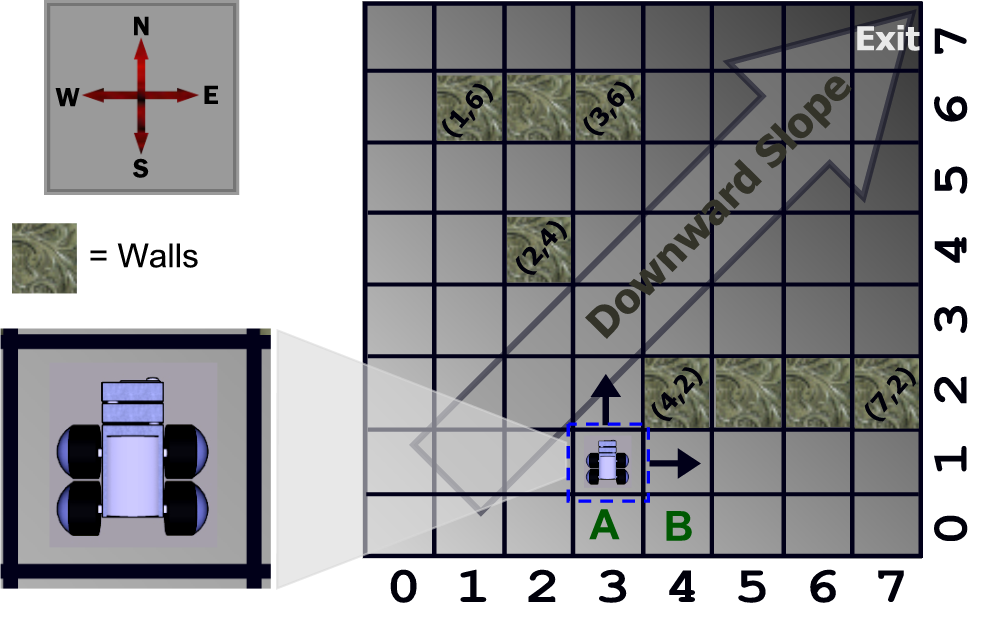
\includegraphics[width=0.75 \textwidth]{6.png}
					\caption{一个可能的局面}
				\end{figure}
				
				$N, M \le \num{1e6}, K \le \num{1e3}$。

			\subsubsection{算法讨论}
				可以得出一个 时间复杂度 $\mathcal{O}\left(N \times M\right)$ 的动态规划。
				\begin{align}
					F[1][M] & = \text{真}\\
					F[i][j] & = (F[i - 1][j] \lor F[i][j + 1]) \land (i, j) \text{ 不是墙}\\
					Ans & = \sum_{F[i][j]\text{ 为真}} 1
				\end{align}
				注意到只有最多 \num{1e3} 堵墙,故将整个平面离散化后,$N, M$ 都会变为  $\mathcal{O}\left(K\right)$ 的,这样这个动态规划就可以在有限的时间内出解了。
			\subsubsection{时空复杂度}
				时间复杂度 $\mathcal{O}\left(K^2\right)$。
					
				空间复杂度 $\mathcal{O}\left(K^2\right)$。
		\newpage
		\subsection{ACM/ICPC World Finals 2010 D Castles}
			\subsubsection{题目大意}
				一个树 $T = (V, E)$,点有三个权 $W_{1, 2, 3}: V \mapsto \mathbb{R}_{+}$。 若干人一起在树上行走,如果走到一个从未访问的点 $x \in V$,那么\emph{必须}访问该节点,并要求此时至少有 $W_1(x)$ 个人,同时会有 $W_2(x)$ 个人死去(并且要求到达时至少有这么多人),并且还要  $W_3(x)$  个人留在这里(人也要够),脱离大部队。访问完所有节点,且所有边两个方向至多走一次。问开始时至少
				要有多少人才能完成任务?起点任意。
				
				点数 $N = |V| \le 100$。
			\subsubsection{算法讨论}
				注意到死去的人和留下的人本质实质上是相同的,都不能帮助拼凑接下来游行的人数,故将其先合并 $\forall x \in V, W_0(x) = W_2(x) + W_3(x)$。
				
				由于所有边两个方向至多走一次,那么旅行的本质实质上是,先从某一节点起访问,然后顺次完整地访问其各个儿子的子树,最后回到此节点%及父节点
				。
				故不妨先枚举起点(即根节点),令 $F[x]$ 表示遍历根为  $x$  的子树至少需要多少人,$G[x]$ 表示遍历根为  $x$  的子树会死(留下)多少人。后者容易求出
				\begin{align}
					G[x] = W_0(x) + \sum_{x\text{ 的儿子}\, y}  G[y]
				\end{align}
				而前者需要求出一个最优的访问儿子的顺序。
				
				不妨假设先求出了以儿子为根的子树的 $F[\cdot], G[\cdot]$,并且得到了一个访问儿子的顺序 $p_1, p_2, ..., p_k$,那么一开始的人数 $x$ 满足
				\begin{align}
					\left\{\setlength{\tabcolsep}{2.5pt}
						\begin{tabular}{rcl}
							$x$ & $\ge$& $W_1(x)$\\
							$x - W_0(x)$ & $\ge$& $ F[p_1]$\\
							$x - W_0(x) - G[p_1]$ & $\ge$& $ F[p_2]$\\
							$x - W_0(x) - G[p_1] - G[p_2]$ & $\ge$& $ F[p_3]$\\
							&  $\cdots$ &  \\
							$x - W_0(x) - G[p_1] - \cdots - G[p_{k-1}]$ & $\ge$&$ F[p_k]$\\
							$x - W_0(x) - G[p_1] - \cdots - G[p_{k}]$ & $\ge$&$ 0$\\
						\end{tabular}\label{D Castles}
					\right.
				\end{align}
				考虑中间的两个相邻方程 $(0 \le i \le k - 2)$
				\begin{align}
							x - W_0(x) - G[p_1] - \cdots - G[p_i] & \ge F[p_{i + 1}]\\
							x - W_0(x) - G[p_1] - \cdots - G[p_{i + 1}] & \ge F[p_{i + 2}]
				\intertext{即}
							x - W_0(x) - G[p_1] - \cdots - G[p_i] & \ge F[p_{i + 1}] \label{DCastlesA} \\
							x - W_0(x) - G[p_1] - \cdots - G[p_i] & \ge G[p_{i + 1}] + F[p_{i + 2}] \label{DCastlesB}
				\end{align}
				如果 $G[p_{i + 1}] - F[p_{i + 1}] \ge G[p_{i + 2}] - F[p_{i + 2}] $ 那么
				\begin{align}
							F[p_{i+2}] \le G[p_{i + 1}] + F[p_{i + 2}] \ge F[p_{i + 1}] + G[p_{i + 2}] \ge F[p_{i + 1}]
				\end{align}
				并交换 $p_{i + 1}, p_{i + 2}$,\label{D Castles A} \label{D Castles B} 变为
				\begin{align}
							x - W_0(x) - G[p_1] - \cdots - G[p_i] & \ge F[p_{i + 2}] \label{DCastlesC}\\
							x - W_0(x) - G[p_1] - \cdots - G[p_i] & \ge G[p_{i + 2}] + F[p_{i + 1}]\label{DCastlesD}
				\end{align}
				\eqref{DCastlesC}  相对于 \eqref{DCastlesB},\eqref{DCastlesD} 相对于 \eqref{DCastlesA} 都更松了,故 $x$ 的解集更大了。
				重复上述过程,直到 $p_i$ 按照  $G[p_{i}] - F[p_{i}]$ 排序,此时  $x$ 的解集最大,且能取到最小值。又因初始序列具有任意性,故此解即为最小解。
				
				故直接排序确定顺序,后参考 \eqref{D Castles} 即可确定 $F[\cdot]$ 的值。最终答案为 $F[\text{根节点}]$ 的最小值。 
			
			\subsubsection{时空复杂度}
				时间复杂度 $\mathcal{O}\left(N^2\log N \right)$。
					
				空间复杂度 $\mathcal{O}\left(N\right)$。
		\newpage
		\subsection{ACM/ICPC World Finals 2010 F Contour Mapping}
				
				\begin{wrapfigure}{r}{0.45 \textwidth}
					\centering
					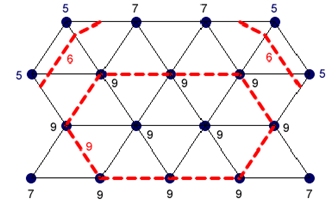
\includegraphics[width=0.4 \textwidth]{7.png}
					\caption{等高线} \vskip-2.5em
				\end{wrapfigure}
			\subsubsection{题目大意}
				如右图的地图,每个实心点都有一个高度,各三角形在空间中过对应点。等高线表示海拔为某高度 $h$ 的整数倍,图形的\emph{轮廓}。求等高线长度。
				
				图形有 $N$ 行,奇数行有 $M$ 列。$N, M \le \num{100}$。$1 \le h \le \num{1000}$,海拔 $\le \num{1e6}$。
			\subsubsection{算法讨论}
				先考虑不过三角形的边界的等高线。由于这一部分等高线就是平面 $z = kh$ 与三角形平面交出的直线,故过三角形的边上的两点。求出三角形边上海拔为 $kh, k \in N^+$ 的点,并将其对应地连接。计算可知同一个三角形内相邻线段长度为等差数列,使用公式求和便知。
					
				对于在三角形边界上的等高线,先需枚举相邻,等高的两点,并判断以其为边界的两个三角形的对点的高度也是均和此边线否一致(须位于图形内)——如果是,那么这条边界不是等高线;反之,是等高线,计入答案。
					
				求和便知。
			\subsubsection{时空复杂度}
				时间复杂度 $\mathcal{O}\left(N \times M \right)$。
				
				空间复杂度 $\mathcal{O}\left(N \times M \right)$。
		\newpage
		\subsection{ACM/ICPC World Finals 2010 J Sharing Chocolate}
			\subsubsection{题目大意}
				有一个 $N \times M$ 网格。你需要用剪刀,每次沿着网格,不拐弯,一刀将其剪成两部分。操作可重复若干次,但最终必切成 $K$ 块,且 $K$ 块的大小须为指定的大小(格子数而非长宽)。问是否有一个可行的操作方案。
				
				$N, M \le 100, K \le 15$。
			\subsubsection{算法讨论}
				动态规划。设 $F[N][S]$ 表示当前需要剪出可重集 $S$ 里的块数,且现在网格长 $N$ 宽 $\sum_{i \in S} i / N$ 的情况下,是否有可行的方案。
				\begin{align}
					F[N][S] &= \text{真}, & |S| = 1\\
					F[N][S] &= \LOR_{\text{枚举裁剪方法,且} \atop \text{剪出一块 $x \in S$}} { F[\text{新尺寸的长度}][S \setminus\{ x\}] }
				\end{align}
				% 此处的求和 $(\sum)$ 表示逻辑析取$(\lor)$。
				
				答案即 $F[N][\text{指定的大小}]$。
			\subsubsection{时空复杂度}
				时间复杂度 $\mathcal{O}\left(N^2 2^K \right)$。
				
				空间复杂度 $\mathcal{O}\left(N 2^K \right)$。
		\newpage
		\subsection{ACM/ICPC World Finals 2010 K Paperweight}
			\subsubsection{题目大意}
给定三维空间中一个有五个顶点的多面体,内部有一个固定点 $A$。请将其放在桌面上,使得即使重心微移了 $\mathbf{\epsilon}, \epsilon \le 0.2$ 后,也仍然稳定(合力矩 $ = \mathbf{0}$),求所有放法中,固定点 $A$ 离桌面的最近和最远距离。

			\subsubsection{算法讨论}
				不妨枚举底面。根据物理知识,力矩平衡当且仅当重心在桌面的投影在支撑面(多面体与桌面接触的面)内。考虑微移 $\mathbf{\epsilon}, \epsilon \le 0.2$,等价于支撑面各边向内平移$ \epsilon$ 单位,方向垂直于边界。直接使用这个进行判断放法的合法性。
				
				枚举底面后,需要计算点面距离。设该面上三个不公线的点 $P, Q, R$,则法向量 $\mathbf{v} = \overrightarrow{PQ} \times  \overrightarrow{PR}$,点面距
				\begin{align}
					\pm d & = \frac{\overrightarrow{AP} \cdot \mathbf{n}}{n} =  \frac{\overrightarrow{AP} \cdot \mathbf{n}}{\sqrt{ {\mathbf{n}}^2 }}  = \frac{\overrightarrow{AP} \cdot \left(\overrightarrow{PQ} \times  \overrightarrow{PR}\right)}{\sqrt{ {\left(\overrightarrow{PQ} \times  \overrightarrow{PR}\right)}^2 }}
				\end{align}
				取 $d$ 的最大最小值即可。
				
				特殊处理退化成四面体的图形(若视为五面体,则有两面都是底面)。
			\subsubsection{时空复杂度}
				时间复杂度 $\mathcal{O}\left(1 \right)$。
				
				空间复杂度 $\mathcal{O}\left(1 \right)$。
		\newpage